%\documentclass[11pt,a4paper]{report}
\documentclass[11pt,a4paper]{article}
%\documentclass[11pt,a4paper]{amsart}

\usepackage{listings}
\usepackage{amsmath}
\usepackage{verbatim}
\usepackage{graphicx}

\lstset{language=Python}

\title{An Optimal Dynamic Metascheduler for Continuously Cycling
Multi-Model Forecasting Systems}

\author{Hilary Oliver, NIWA}

\begin{document}

\maketitle

\begin{abstract} A metascheduler is a control system that determines
    when members of a set of tasks with dependencies are {\em ready} to
    be scheduled for execution.* This paper describes a flexible
    metascheduling algorithm that provides optimal control over
    continuously cycling multi-model environmental forecasting systems
    without prescribing task execution order or requiring that
    dependencies between tasks be explicitly defined. Each task simply
    registers its own prerequisites, without reference to other tasks in
    the system, and dependencies are negotiated dynamically as outputs
    are reported so that correct execution order emerges naturally at
    run time.  The algorithm is optimal in the sense that tasks are
    queued for execution as soon as their prerequisites are satisfied
    regardless of associated forecast cycle or any other consideration.
    Tasks from many different forecast cycles can therefore run
    simultaneously, where dependencies allow, to achieve maximum
    throughput during catch up from delays or when running the entire
    system over historical case study periods, and can allow new kinds
    of real time operation. The absence of any task-specific scheduling
    logic or predefined dependencies lends great flexibility: tasks can
    be switched on and off on the fly, new tasks can be added without
    altering the main program, and parallel test systems that feed off
    the main operation, or entirely new systems, can be built quickly.
    Our dynamic metascheduler, {\em sequenz}, is easily interfaced to
    existing tasks (models etc.). It is written in the Python language
    and uses the Python Remote Object protocol ({\em Pyro}) to control
    tasks on multiple platforms at once. 

*The term can also refer to {\it a single aggregate view of multiple
Distributed Resource Managers}, which is not the topic of this paper.

\end{abstract}

\pagebreak
\tableofcontents
\pagebreak

\section{Cycling Multi-Model Forecasting Systems}

Continuously cycling multi-model environmental forecasting operations
generate forecast products at regular intervals using a set of connected
scientific models and associated data processing tasks\footnote{A {\em
task} is any group of processes treated as a single entity for
scheduling purposes.} driven by real time observational data and/or
forecast fields from another operation. The EcoConnect Forecasting
System at the National Institute of Water and Atmospheric Research
(NIWA) in New Zealand takes real time atmospheric and stream flow
observations, and operational global weather forecasts from the UK Met
Office, and uses these to drive global sea state and regional data
assimilating weather models, which in turn drive regional sea state,
storm surge, and catchment river models, plus tide prediction, and a
large number of associated data collection, quality control,
preprocessing, postprocessing, product generation, and archiving
tasks.\footnote{Plans for EcoConnect include additional deterministic
regional weather models and a statistical ensemble of weather models.}
In real time operation, the arrival of new external driving data
initiates a new {\em forecast cycle} consisting of a set of tasks with a
common {\em forecast reference time}, the nominal start time of the new
model forecasts. Not all tasks necessarily run in every cycle: the
regional weather model in EcoConnect runs four times daily in the 00,
06, 12, and 18 UTC cycles, but it supplies surface pressures to a
regional storm surge model that runs only twice daily, in the 00 and 12
UTC cycles, and precipitation accumulations to catchment river models
that run on an hourly cycle as they assimilate real time stream flow
observations. 

\subsection{Sequential Cycling}

In real time operation a new forecast cycle is initiated by the arrival
of the next batch of external driving data, at which point the previous
cycle must be well finished (otherwise the system would get increasingly
further behind with each cycle). Strictly speaking there are
dependencies between forecast cycles that must be respected (in other
words a task that takes input from a previous cycle must not be executed
before that input has been generated) but these can be treated as
implicitly satisfied, and therefore ignored, in real time
operation.\footnote{But note that our new control system allows new
kinds of real time operation that violate this; e.g.\ the way that
EcoConnect's TopNet catchment model depends on the regional weather
forecast.} Consequently it is natural to think of forecasting systems as
consisting of a linear series of distinct forecast cycles. Indeed, as
far as the author is aware all existing control systems do assume this
behaviour - although it is difficult to be sure because they are
invariably highly system-specific in-house designs that are not
documented in the literature.\footnote{DAGMan, which is part of the
Condor distributed workload management system [REF:...], is a
metascheduler for jobs with dependencies, but it does not appear
to be suited to continuous dependent systems.} 

\subsection{Interleaved Cycling}

If the next external driving data are available in advance of the
current cycle finishing, as frequently happens after breakdowns and
delays, it may be possible to start the next cycle before the current
one is finished, in which case maintaining strict sequential cycling
seems an unnecessary impediment.  This is a serious problem for complex
operations like EcoConnect that have little downtime between forecast
cycles and consequently take much longer than necessary to catch up
after delays.  But to realize the potential for functional parallelism
the aforementioned intercycle dependencies must be handled properly so
that tasks are never executed before their inputs, if any, from earlier
cycles have been generated. The simplest kind of intercycle dependence
is that which connects consecutive runs of most forecast models: each
forecast generates a ``background state'' valid at the start of the next
forecast and used in initialising it. It is also possible (if using our
new control system, at least!) to have dependencies that span more than
one forecast cycle and connect different task types; e.g.\ the
EcoConnect catchment model's dependence on the regional weather model,
as described later. 

\section{Metascheduling By Example}

A control system for a forecasting operation should ideally queue each
task for execution as soon as its prerequisites are satisfied. Whether
queued tasks acutally begin executing immediately depends on resource
availability as determined by the batch queue scheduler(s), but in any
case this the best that can be done. 

\begin{figure} 
    \begin{center}
    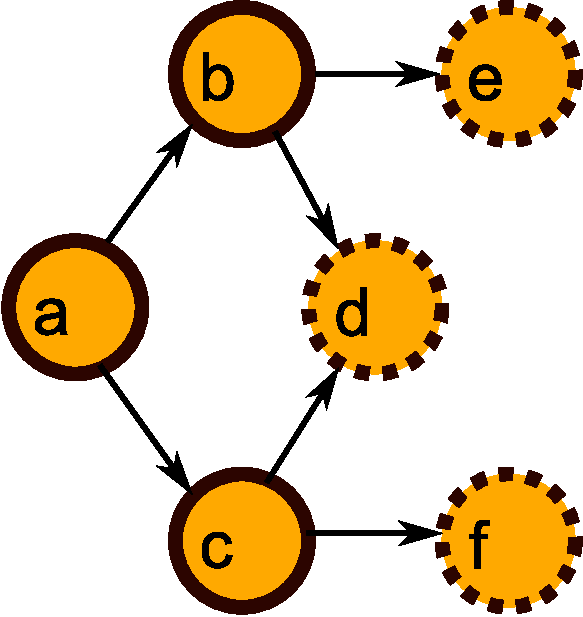
\includegraphics[width=4cm]{dependencies-one} 
    \end{center}
    \caption{\small Dependency diagram for a single forecast cycle in a
    simple example system. Tasks {\em a, b,} and {\em c} represent
    forecast models, and {\em d, e} and {\em f} are post processing or
    product generation tasks.} 
    \label{fig-dep-one} 
\end{figure} 

Figure \ref{fig-dep-one} shows a dependency diagram, which forms a
{\em Directed Acyclic Graph}, for a single cycle of a simple example
system consisting of three forecast models ({\em a, b,} and {\em c}) and
three post processing or product generation tasks ({\em d, e} and {\em
f}).  Within the same forecast cycle each task may depend on one or
more other ``upstream'' tasks, and may itself be depended on by one or
more other ``downstream'' tasks.  A control system should therefore be
capable of managing, within a single forecast cycle, multiple parallel
streams of execution that branch when one task generates output for
several downstream tasks, and merge when one task takes input from
several upstream tasks. 

\begin{figure}
    \begin{center}
        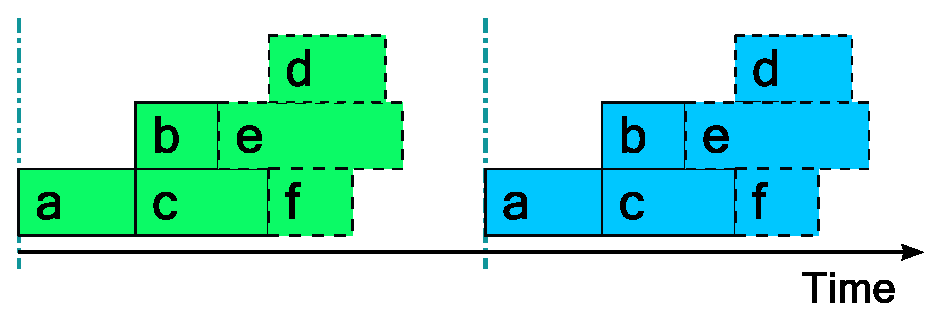
\includegraphics[width=8cm]{timeline-one}
    \end{center}
    \caption{\small Optimal job schedule for two consecutive cycles of
    the example system during real time operation. Execution times are
    represented by the horizontal extent of the task bars, and the gray
    area is downtime while the system waits on new external driving
    data.  A vertical section through the graph will intersect all tasks
    executing at the same time, but the vertical ordering of tasks is
    not meaningful.}
    \label{fig-time-one}
\end{figure}

Figure \ref{fig-time-one} shows two consecutive cycles of the optimal
job schedule for the example system in real time operation, given task
execution times represented by the horizontal extent of the bars. It is
optimal in the sense that every task begins executing as soon as its
prerequisites are satisfied. There is a gap as the system waits on
external driving data for the next cycle.  All prerequisites here
involve upstream tasks {\em finishing} rather than intermediate
outputs,\footnote{Model background states are written early in a
forecast, assuming the forecast length is much longer than the forecast
cycle period, so in principle forecast models don't actually have to
wait on their previous instance {\em finishing} - the new system could
easily handle this using ``background state ready'' messages instead 
``task finished'' messages to trigger task abdication; more on this
later.} but this is merely a simplification that makes for clearer
diagrams.  

The dependency graph of Figure \ref{fig-dep-one} is technically
incomplete because it does not show any intercycle dependencies.  As
discussed above, ignoring these is equivalent to requiring sequential
cycling at all times. In that case Figure \ref{fig-time-one-a} shows the
best that can be done, in general, to catch up from delays. For a
particular set of tasks there could be a point at which consecutive
cycles can be allowed to simply overlap without violating any
dependencies, but that would have to be determined anew every time 
the system changes, and we are interested in automatic optimal
interleaving of forecast cycles regardless of the task list.  

\begin{figure}
    \begin{center}
        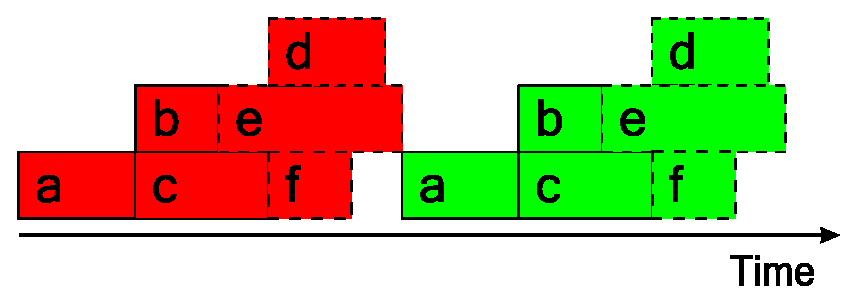
\includegraphics[width=8cm]{timeline-one-a}
    \end{center}
    \caption{\small Job schedule for two consecutive cycles of the
    example system during catch up from a delay. This is the best
    that can be done in the general case if intercycle dependencies
    are not taken into account.}
    \label{fig-time-one-a}
\end{figure}

\begin{figure} \begin{center}
    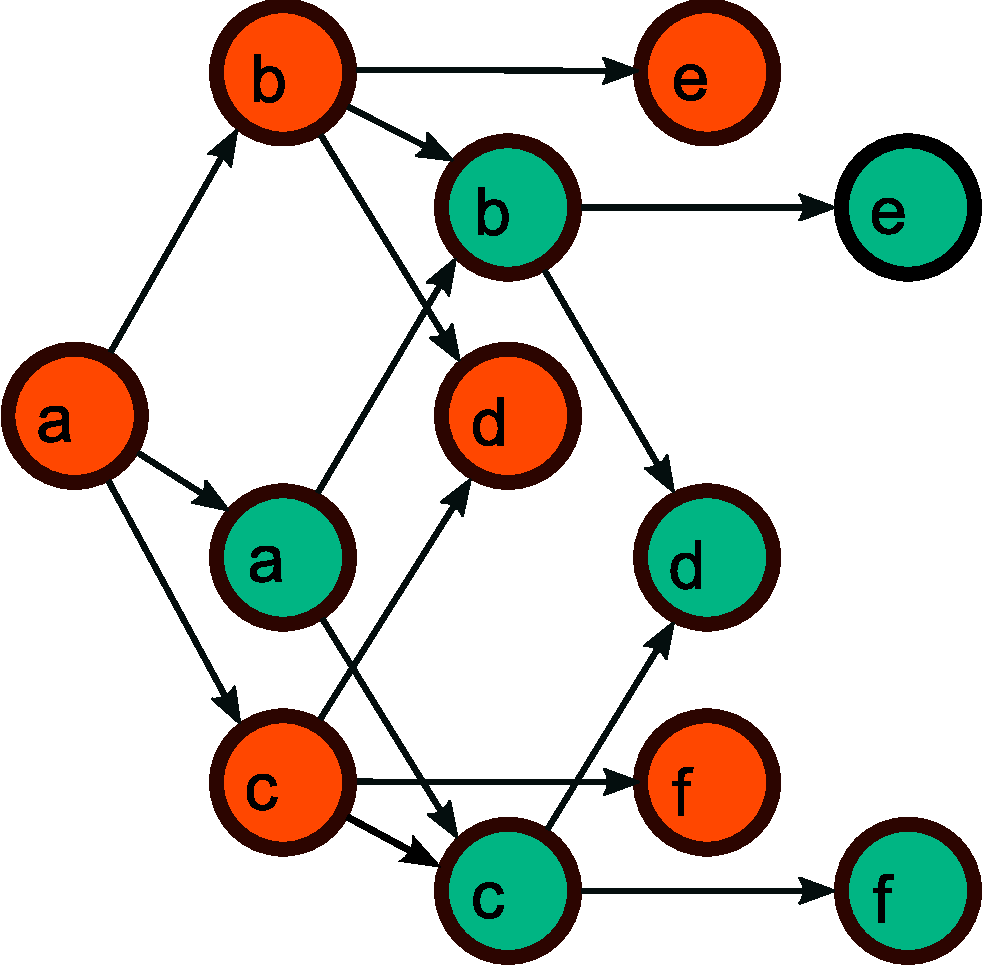
\includegraphics[width=6cm]{dependencies-two} \end{center}
    \caption{\small Complete dependency graph for the example
    system, assuming the least possible intercycle dependence: the
    forecast models ($a$, $b$, and $c$) depend on their own previous
    instances. The dashed arrows show connections to previous and
    subsequent forecast cycles.} 
    \label{fig-dep-two}
\end{figure}

Figure \ref{fig-dep-two} shows the complete dependency graph for the
example system, assuming the least possible intercycle dependence: each
of the model forecasts ($a$, $b$, and $c$) depends on their own previous
instance. Real systems can have other more complex dependencies too, as
noted above, but this minimal set is sufficient to demonstrate the
benefits of handling intercycle dependencies.

\begin{figure} 
    \begin{center} 
        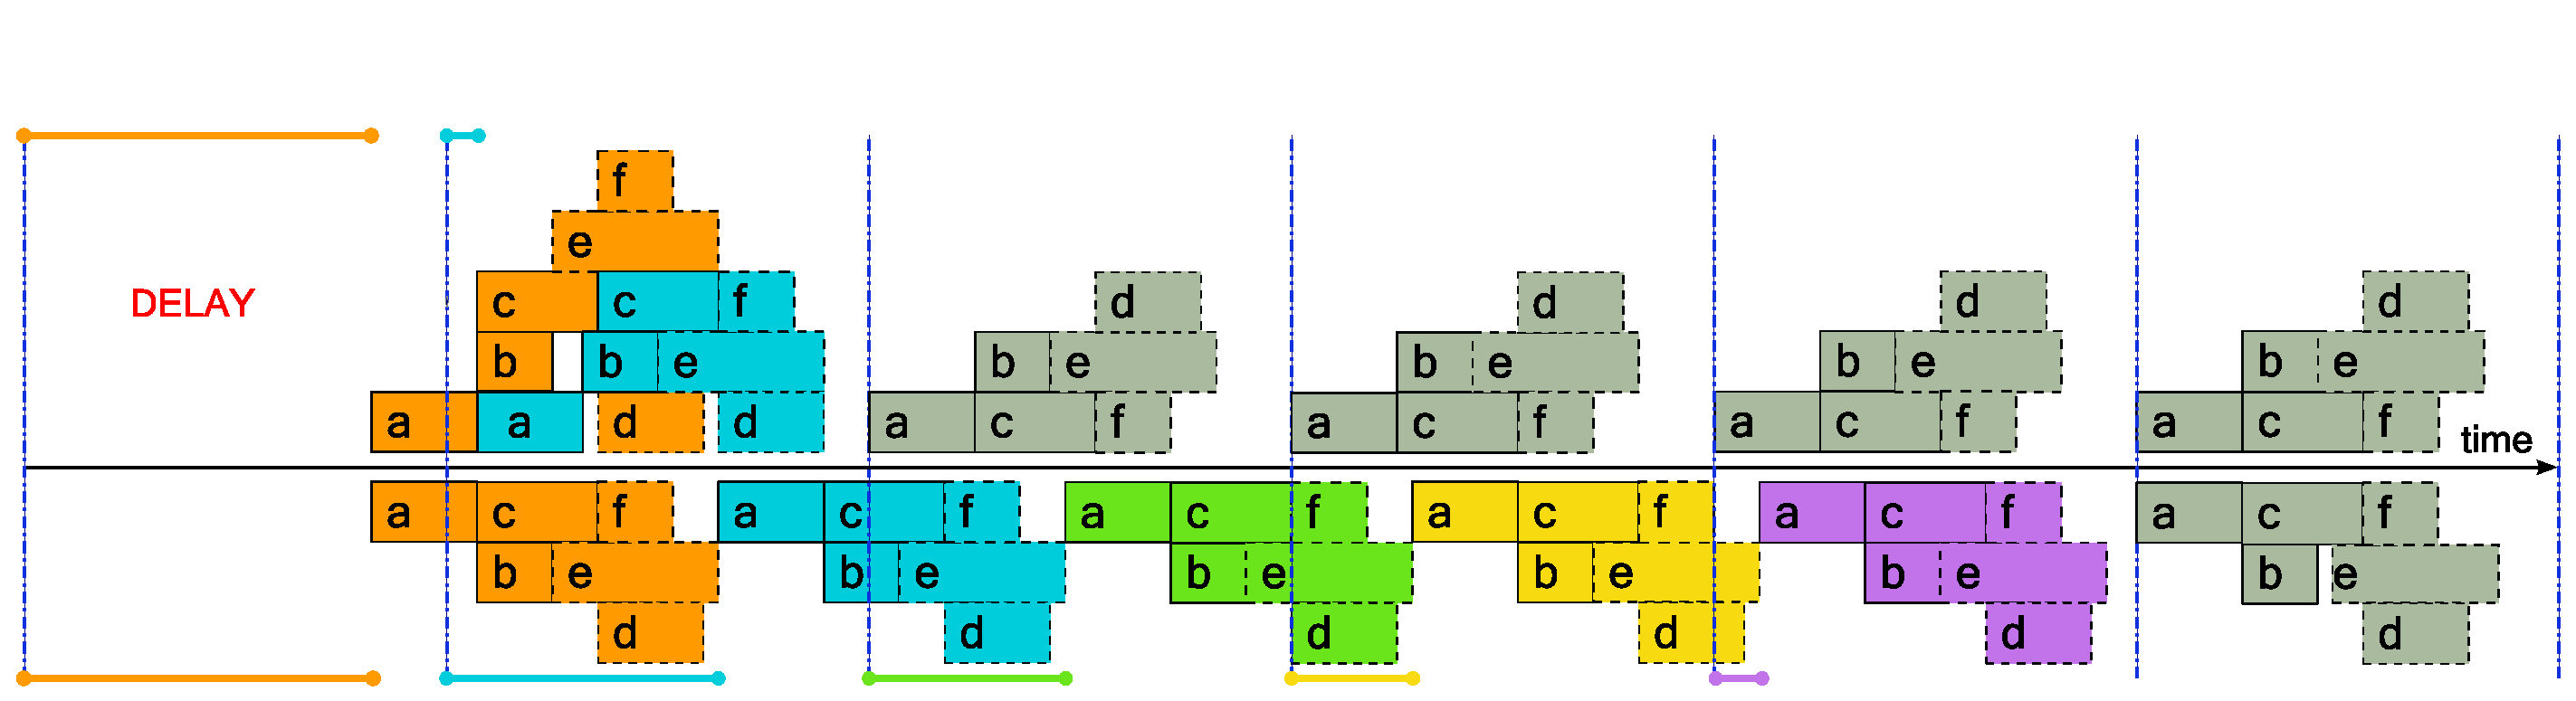
\includegraphics[width=12cm]{timeline-three}
    \end{center} 
    \caption{\small Job schedules for the example system after a 
    delay of almost one whole forecast cycle, when intercycle
    dependencies are taken into account (above the time axis), and when
    they are not (below the time time axis). The colored lines indicate
    the time that each cycle is delayed, and normal ``caught up'' cycles
    are shaded gray.} 
    \label{fig-time-three}
\end{figure} 

Figure \ref{fig-time-three} shows job schedules for the example system
after a delay of almost one forecast cycle. When intercycle dependencies
are taken into account it can be seen that the cycle immediately after
the delayed one is almost unaffected, and subsequent cycles all run on
time. With strict sequential cycling, on the other hand, it
takes many cycles for the system to catch up. Note that simply
overlapping the normal single cycle schedule after the delay, from the
same start point, would result in dependency violations.

\begin{figure} 
    \begin{center} 
        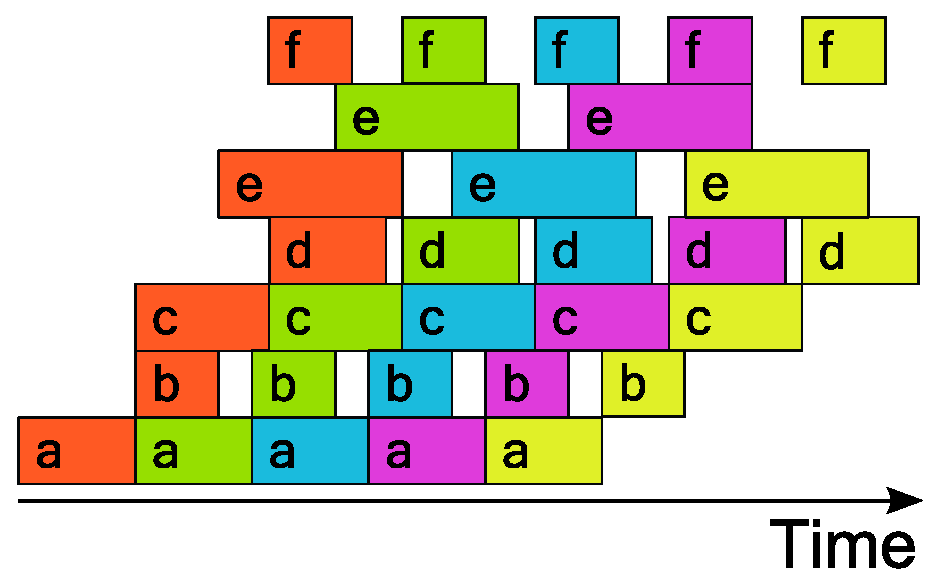
\includegraphics[width=8cm]{timeline-two}
    \end{center} 
    \caption{\small Job schedules for the example system in case study
    mode, or after a long delay, when the external driving data are
    available many cycles in advance. Above the time axis is the optimal
    schedule obtained when the system is constrained only by its true
    dependencies, as in Figure \ref{fig-dep-two}, and underneath it is
    the best that can be achieved when intercycle dependencies are
    ignored.} 
    \label{fig-time-two}
\end{figure} 

Similarly, Figure \ref{fig-time-two} shows job schedules for the example
system in case study mode (or when catching up after a very long delay)
when the external driving data are available many cycles in advance. The
initial task {\em a}, which is likely to be a resource intensive
atmosphere or ocean model, has no dependence on cotemporal upstream
tasks and can therefore run continuously, regardless of how much
downstream processing is yet to be completed in its own cycle or in any
previous forecast cycle. In practice initial forecast tasks would depend
on cotemporal upstream tasks that wait on the external driving data, but
they will return immediately when the external data is already
available, so the result stands. Other tasks can cycle at regular short
intervals, the interval depending on [CHECK THIS] the task run length
relative to that of its longest cotemporal upstream dependency path. In
this case {\em c} can also run continuously, and consecutive instances
of {\em e}, which is a post processing task with no previous-instance
dependence, can actually overlap. Tasks from three or four different
cycles run simultaneously at any given time, even for this very simple
example, and system efficiency is clearly far in advance of that of the
sequential cycling schedule.  


\section{Sequential Cycling Implementation}

Realistic systems are likely to have many more tasks than our example
system, but the dependency graphs should be qualitatively similar. The
obvious control system design candidate for Figure \ref{fig-dep-one}
is a Finite State Machine that, within an event loop that responds to 
tasks finishing and/or completion of important task outputs, enforces
a predetermined non-linear order of events using hard coded scheduling
logic.  For the example system, it might look something like this:

{\small
\noindent
\rule{5cm}{.2mm}
\begin{lstlisting} 

when an_output_was_just_completed():

    if A.just_finished():
        B.start_executing()
        C.start_executing()

    elif B.just_finished():
        E.start_executing()

    elif C.just_finished():
        F.start_executing()

    elif B.just_finished() and C.already_finished()
        or
         C.just_finished() and B.already_finished(): 
        D.start_executing()
\end{lstlisting}
}

As far as the author is aware all existing forecast control systems are
variants of this design, or an even simpler one in which the user has to
explicitly define the task execution order, perhaps with some crude
means of specifying functional parallelism as well. Even as a single
cycle algorithm the Finite State implementation suffers from being
highly system-specific and the logic becomes increasingly convoluted as
system complexity increases. This inevitably leads to inflexibility and
fragility (consider adding a new task with dependencies into an existing
system), and extending the design to continuous complex networks with
intercycle dependencies hardly seems possible, even for our simple
example system.


\section{Interleaved Cycling Implementation}

In this section we describe a novel algorithm that achieves optimal
continuous metascheduling as in Figures \ref{fig-time-two} and
\ref{fig-time-three}, and smoothly transitions to a linear sequence of
distinct forecast cycles as in Figure \ref{fig-time-one}, as the system
catches up to real time.  

\subsection{The Basic Algorithm}

From the discussion above it is apparent that the additional complexity
due to explicitly handling intercycle dependencies is too difficult to
deal with in a Finite State Machine, and that the ``forecast cycle'' as
a global control system parameter has to be replaced with an independent
``forecast reference time'' for each task. This devolving of cycle
timing to the individual tasks suggests treating the system as a {\em
simulation} of autonomous proxy objects that represent the external
tasks and interact regardless of reference time to negotiate
dependencies at run time (i.e.\ by matching completed outputs against
prerequisites). If this can be made to work it provides extraordinary
power and flexibility because it treats all dependencies equally and it
makes any convoluted task scheduling logic entirely disappear: if task
proxy objects can interact indiscriminately then they don't need to know
{\em who} is supposed to satisfy their prerequisites and they can be
defined without reference to the other tasks in the system (except of
course that some other task(s) must exist that will satisfy their
prerequisites).  Existing tasks could be taken out of the system, or new
ones added, without changing the control system in any other way.
Further, by means of object polymorphism\footnote{Polymorphism is the
ability of one type to appear as and be used like another type. In OOP
languages with inheritance, this usually refers to the ability to treat
derived class objects as if they were members of a base class so that,
for instance, a group of mixed-type objects can all be treated as
members of a common base class while retaining their specialized derived
class behaviour.} the control system can be designed to automatically
handle any future task so long as it is derived from (inherits the
properties of) the original task base class.

The following simple description should be sufficient to enable the
reader to understand how the algorithm achieves optimal forecast
cycle-independent metascheduling. Everything else is arguably just
implementation, although some important aspects of that are not trivial
and will be discussed later.

\begin{itemize}

    \item The control system maintains a pool of autonomous {\em task
        proxy objects} that represent each real task. 
       
    \item The internal state of a task proxy object must reflect that
        of the real task it represents. This state information includes:

        \begin{itemize}

            \item task proxy object name.

            \item associated external (real) task.  

            \item owner of the real task, if necessary (who the task
                should run as).

            \item UTC {\em forecast reference time}, e.g. $2010012418$
        
            \item current execution status: {\em waiting}, {\em running}, 
                {\em finished}, or {\em failed}. 

            \item a list of prerequisites and whether or not they are
                satisfied yet, e.g.\ {\em file FOO is ready}. 

            \item a list of outputs completed so far, e.g.\ {\em file
                FOO is ready}.

        \end{itemize}
       
    \item A task proxy object can launch its associated external task
        when all of its prerequisites are satisfied.

    \item A task proxy object can interact with other task proxy
        objects (regardless of reference time; all dependencies are now
        equal) to determine if any of their completed outputs can
        satisfy any of its prerequisites.

    \item The control system gets the task pool to interact and
        negotiate dependencies whenever any new output is reported.
 
    \item A task proxy object must exist by the time it is needed to
        interact with other tasks, and must not cease to exist before
        it is no longer needed.

\end{itemize}

\subsection{Task Proxy Object Life Cycle}

blah.

\label{sec-task-messaging}

\subsection{Coupling Task Proxies to Tasks} 

Our task proxy objects must keep track of progress in their external
counterparts. Most task prerequisites are just files generated by other
tasks, so it is tempting to have the controller use the appearance of
expected new output files as a proxy for task progress. But we have to
be sure that a newly detected file is complete, not just that it exists,
and it is difficult to do this in an OS-independent way (using {\em
inotify} on Linux, for example.). 
%On Linux one could insist that every completed output file is
%immediately renamed by the generating task, and have the controller use
%{\em inotify} to watch for the sudden appearance of the new file
%(because file rename operations are atomic when the source and target
%are on the same file system) [REF: Simon, if he wants]. But this is not
%platform independent, and most forecast systems run on heterogeneous
%distributed hardware. 
More importantly though, prerequisites are not necessarily single files:
a task could conceivably depend on completion of a large set of files, a
database update, or a data transfer by remote procedure call, for
instance. Consequently we chose to use a high level messaging system for
communication between external tasks and the control system. This is
platform independent and allows tasks to be triggered off any
conceivable condition. For example, rather than detecting the existence
of the file {\em FOO}, the controller would receive a message saying
{\em file FOO is ready}, or similar, from the task that has
just generated the file.  There is no need for the control system itself
does to verify that the message is true (i.e. that file {\em FOO}
really does exist) because any downstream task that
depends on file {\em FOO} must necessarily do that itself, and error 
conditions can be reported back to the controller, and possibly to a
separate monitoring system as well, at that point.

The Python Remote Object Protocal (Pyro) allows external programs to
communicate directly, across the network, with specific objects inside
the running controller. This means that tasks can communicate directly
with their own proxy objects, obviating the need for any any internal
message brokering mechanism in the control system.    

Each task must express its prerequisites (i.e.\ its dependence on
upstream tasks) as a text string, for example ``file X is ready'', or
``task X has completed'', or ``task X has completed writing all Y
files'', and must send messages of the same kind back to the controller
to indicate when it has reached an important waypoint or completed
generated any important outputs.  

\subsection{Logging}

blah.


\subsection{Pyro}

blah.

\subsection{Pure Simulation Mode}

blah.

\subsection{System and Task Definition}


\begin{comment}

there are several kinds of non-cotemporal (different reference time)
dependence.  Forecast models depend on their own previous instance,
because one forecast generates the {\em background model state} for the
next.  In addition, some forecast models may depend explicitly on
earlier tasks of a different type, as well as on their own previous
instance.  Post processing tasks, on the other
hand, do not depend on their own previous instance, strictly speaking,
but they depend on cotemporal forecast models that do. EcoConnect's
hourly river flow forecasts, for example, take input from the most
recent previous regional weather forecast.  Finally, some tasks, such as
those that wait on external input data, and tide models, may have no
upstream dependencies at all.

Non-forecast model tasks can even overlap with their own previous
instances, if the opportunity arises (this occurs when a post processing
task takes longer to run than the delay between its upstream model
starting and it starting).  System throughput can be greatly increased
by allowing tasks from many different forecast cycles to run
simultaneously where dependencies allow.

This could be done by checking for the existence of required inputs
directly, or by monitoring the state of the other tasks that are known
to provide the inputs in each case (are they finished yet?).  

\subsection{Dynamic Metascheduling}

knows its own prerequisites (inputs) and outputs, and can interact
with other tasks to negotiate dependencies so that correct scheduling
emerges naturally at run time.  The entire scheduling problem is now
contained within the task interaction step, which is almost trivial
because it is completely indiscriminate: whenever any task changes
state, {\em each task} asks {\em all the others} if they can satisfy its
prerequisites with their completed outputs (it does not matter that most
of these interactions are destined to be fruitless). The control program
thus remains simple and generic, regardless of the number of tasks or
the complexity of their interdependencies; it simply manages a set of
tasks that are all individually configured as if they were to run in
isolation.\footnote{The system manager does of course have to ensure
that the configured task pool is self consistent, i.e.\ that each task's
prerequisites will be satisfied by some other task(s) in the system.}
The total absence of explicit scheduling logic makes this method
extremely flexible and extensible.\footnote{To extend the system, one
simply derives a new class definition that lists the new task's
prerequisites and outputs. The new task will automatically run at the
right time, i.e.\ when its prerequisites have been satisfied by some
other task(s) in the system.}

Dynamic scheduling can be viewed as a simulation of an interacting task
set in which the state of each {\em simulee} is tied to, and can
influence, that of the real task it represents.  This suggests a
powerful dummy mode of operation in which the simulation is divorced
from reality by replacing external tasks with an external dummy program
that masquerades as a real task by ``completing'' each of its outputs in
turn (i.e.\ it reports they are complete because, as far as the
controller is concerned, task outputs are just {\em messages}; more on
this below).  The control program cannot distinguish this from real
operations, so the dummy mode allows complete testing of the control
system for a given configured task set, without running any real tasks.


\subsection{{\em Sequenz}}

A dynamic scheduling controller would clearly be most naturally
implemented in an object oriented programming language, which provides
the tools for object construction and interaction.  We must also provide
the means for task objects to launch their external tasks when their
prerequisites are satisfied (e.g.\  by submission to a batch queue
scheduler on a task-dependent target machine), and for synchronization
of the internal states of task objects and the external tasks they
represent, via remote method calls or something similar.  Finally, the
generic description above assumes that task objects exist whenever they
are needed (for external task control and for interacting with other
dependent tasks), so we must devise a task management scheme governing
the creation and destruction of task objects, to ensure that this is the
case.

NIWA's EcoConnect Forecasting System, described above, is controlled by
an asynchronous dynamic scheduling implementation called {\em Sequenz},
implemented in object oriented Python and using the Python Remote Object
protocol ({\em Pyro}) for direct network communication between task
objects and the tasks they represent. It allows tasks from many
different forecast cycles to run at once, where dependencies allow,
transitions seamlessly from ``catchup'' or case study mode (where all
external input is available from the outset and much asynchronous
activity is therefore possible, e.g.\ after system downtime; in this
case) to real time operation, tasks can be switched on and off while the
controller is running, new tasks added without any change to the main
program, and the system can be restarted in arbitrarily complex states
after downtime.  It also features the powerful dummy mode described
above, for testing, and allows easy construction of ad hoc parallel test
systems feeding off the main operational system. Pyro also enables
efficient RPC-based remote control and system monitoring by external
programs.  Sequenz can be interfaced to existing models and tasks with
minimal overhead. 

The operation runs on heterogenous distributed
hardware, which includes a massively parallel supercomputer and several
Linux servers. 

\subsubsection{Applicability}

The dynamic scheduling concept is very general and could in principle be
implemented for any set of interdependent tasks. Sequenz, however, is
somewhat specialized toward cycling forecast systems, such as
EcoConnect, in which each task has an associated {\em reference time}
(generally the nominal forecast start time, or {\em analysis} time, of
the associated forecast model) that all task prerequisites and outputs
depend on in some way. and a set of valid times for each task type (e.g.\
the atmospheric model might run at 00, 06, 12, and 18 UTC each day,
while the river model runs hourly).  One-off task pools with no
particular time dependence, however, are much simpler than this, and it
would not be difficult to strip all reference time handling from the
program.

In addition, EcoConnect operates in a well defined environment so that,
for example, each task knows exactly what its input files look like
(filenaming conventions) and where to get them from (e.g.\ {\em task X}'s
output directory). Consequently, for file-based prerequisites, the
controller does not need to know the file's actual location or check for
its existence, because the external tasks already do that. It could,
however, easily be made to pass file locations between tasks so that all
input/output filenames and paths could be defined centrally in the
control program itself.  



\section{Implementation}

To implement dynamic scheduling we need a specific {\em task management}
scheme that controls when tasks will be created and destroyed, and so
on. There are many options here; for instance: should tasks be created
all at once, in cotemporal batches, or one at a time as their
predecessors finish? The consequences of these choices must be evaluated
carefully, which isn't easy in light of the inherent complexity of
asynchronous operation. At the simpler end of the task management
spectrum we could, for example, create a whole month's worth of tasks at
once and let them interact until everything runs to completion.  Nothing
would run out of sequence, {\em but} system monitoring would be
difficult because of the sheer number of tasks involved, the end of the
month would present an artificial barrier to operations, tasks that lack
prerequisites would all want to run at once, and system restarts would
be overly complicated. 

\subsection{Main Algorithm}

The algorithm below operates on a single pool of interacting task
objects, has simple start up and continuous operation, and is relatively
easy to monitor (task objects exist by the time they are needed but not
for too long before that, and not for too long after they are finished). 

The simplicity of the dynamic scheduling algorithm is clear from the
following code listing, taken directly from the main program:

{\small
\noindent
\rule{5cm}{.2mm}
\begin{lstlisting}
# (startup initialization code omitted)

while True: # MAIN LOOP

   if task_base.state_changed:
       # PROCESS ALL TASKS whenever one has changed state
       # as a result of a remote task message coming in: 
       # interact, run, create new, and kill spent tasks
       #---
       task_pool.process_tasks()
       task_pool.dump_state()
       if task_pool.all_finished():
           clean_shutdown( "ALL TASKS FINISHED" )

    # REMOTE METHOD HANDLING; handleRequests() returns 
    # after one or more remote method invocations are 
    # processed (these are not just task messages, hence 
    # the use of task_base.state_changed above).
    #---
    task_base.state_changed = False
    pyro_daemon.handleRequests( timeout = None )

# END MAIN LOOP
\end{lstlisting}
}

\subsection{Details}

\subsubsection{Startup and Initialization}

An initial reference time and list of task object names are read in from
the config file, then each task object is created at the initial
reference time {\em or} at the first subsequent reference time that is
valid for the task type. Optionally, we can tell the controller to
reload the current state dump file (which may have been edited); this
will override the configured start time and task list. After startup,
new tasks are created only by {\em abdication} (below).

An initial run through the {\em task processing} code, by virtue of the
fact that the main loop starts with task processing, causes tasks with
no prerequisites (e.g.\ {\em downloader}) to enter the {\em running}
state and launch their external tasks immediately. Otherwise ({\em or}
if there are no tasks that lack prerequisites) nothing will happen.



\subsubsection{Creation of New Tasks}

New tasks are created by abdication, i.e.\ create $foo(T\negmedspace
+\negmedspace 1)$ if $foo(T)$ is {\em finished}.  Task abdication
ensures that $foo(T\negmedspace +\negmedspace 1)$ won't run before
$foo(T)$ finishes, without imposing explicit intercycle prerequisites
that would require special treatment at startup (when there is no
previous cycle).  It also ensures that tasks with no prerequisites, e.g.\
{\em downloader} and {\em nztide}, won't all try to run at once.
Tasks are not deleted immediately on abdication (see below).


\subsubsection{Task Interaction} 

Each task keeps track of which of its postrequisites are completed, and
asks the other tasks if they can satisfy any of its prerequisites.  The
fact that task objects do not need to know who is supposed to satisfy
their prerequisites (because they can ask, indiscriminately, every other
task in the system) makes the task interaction (scheduling!) algorithm
almost trivial. The fact that most of these interactions are fruitless
is of no consequence. 

{\small
\noindent
\rule{5cm}{.2mm}
\begin{lstlisting}
class task_pool( Pyro.core.ObjBase ):
    # ...
    def interact( self ):
        # get each task to ask all the others if 
        # they can satisfy its prerequisites
        #--
        for task in self.tasks:
            task.get_satisfaction( self.tasks )
    # ...
\end{lstlisting}
}

\subsubsection{Running Tasks}

Each task object can launch its associated external task, and enter the
{\em running} state if its prerequisites are all satisfied, any existing
older tasks of the same type are already {\em finished}, and fewer than
{\em MAX\_ RUNAHEAD} finished tasks of the same type still exist (this
stops tasks with no prerequisites from running ahead indefinitely).

\subsubsection{Pyro Remote Method Calls}

The Pyro request handling loop executes remote method calls coming in
from external tasks, and returns after at least one call was handled.
Pyro must be run in non-default single-threaded mode (see Appendix
\ref{pyro-appendix}).

\subsubsection{Dumping State} 

The current state (waiting, running, or finished) of each task is
written out to the {\em state dump file}.  This provides a running
snapshot of the system as it runs, and just prior to shutdown or
failure. The controller can optionally start up by loading the state
dump (which can be edited first). Any 'running' tasks are reloaded in
the 'waiting' state.

\subsubsection{Removing Spent Tasks} 

A task is spent if it finished {\em and} no longer needed to satisfy the
prequisites of any other task. Most tasks are only needed by other
cotemporal downstream tasks; these can be removed when they are finished
{\em and} older than the oldest non-finished task. For rare cases that
are needed by tasks in later reference times (e.g.\ nzlam post
processing: multiple hourly topnet tasks need the same most recent
previously finished 06 or 18Z nzlam post processing task), each
non-finished task reports its {\em cutoff reference time} which is the
oldest reference time that may contain tasks still needed to satisfy its
own prerequisites (if it is waiting) or those of its immediate
post-abdication successor (if it is running already), then the task
manager can then kill any finished tasks that are also older than the
oldest task cutoff time.

\subsubsection{Removing Lame Tasks} 

Tasks that will never run (because their prerequisites cannot be
satisfied by any other task in the system) are removed from the {\em
oldest batch} of tasks.  If not removed they would prevent the spent
task deletion algorithm from working properly. Lame tasks can only be
detected in the oldest task batch; in younger batches some tasks may yet
appear as their predecessors abdicate.

Lame tasks are abdicated rather than just deleted, because their
descendents will not necessarily be lame: e.g.\ if the system is started
at 12Z with topnet turned on, all topnet tasks from 12Z through 17Z will
be valid but lame, because they will want to take input from a
non-existent nzlam\_post from 06Z prior to startup. However, the
presence of lame tasks may indicate user error: e.g.\ if you forget
to turn on task type $foo$ that supplies input to task type $bar$,
any instance of $bar$ will be lame.


\subsection{Dummy Mode}

Dummy mode allows complete testing of the control system without running
any real external tasks\footnote{The only difference between dummy mode
and real operation, as far as the controller is concerned, is that
external dummy tasks are not delayed by resource contention.}. When it
is ready to run, a task object will launch an external dummy program
that (i) gets a list of postrequisites from the parent task object and
then (ii) reports back that each one is satisfied at the (estimated)
right time relative to an accelerated dummy clock. Dummy tasks therefore
complete in approximately the same dummy clock time as the real tasks do
in real time. An initial dummy clock offset relative to the initial
reference time can also be specified, which allows simulation of the
transition between catchup and real time operation. Log messages are
stamped with dummy clock time instead of real time.

The same script is used for all external dummy tasks but it has special
behaviour in certain cases: the dummy downloader ``waits for incoming
files'' until 3:15 past its reference time, and the dummy topnet ``waits
for stream flow data'' until 0:15 past its reference time.

The dummy clock can be bumped forward a number of hours by remote
control, while the system is running. This affects the postrequisite
timing of running tasks correctly, but if it causes a running task to
finish immediately the next task in line will still start from the
beginning no matter how big the bump.


\appendix

\section{Essential OOP Concepts}

The simplicity of the dynamic scheduling implementation in {\em sequenz}
is critically dependent on the {\em polymorphic} nature of the {\em task
objects} in the program.  This section contains a minimal introduction
to these Object Oriented Programming concepts.  Refer to any OOP
reference for more detail.

\subsection{Classes and Objects}

A {\em class} is essentially a generalisation of {\em data type} to
include {\em behaviour} (i.e.\ functions or {\em methods}) as well as
state.  {\em Objects} are more or less self contained {\em instances} of
a class. For example, a $shape$ class could define a $position$ data
member that describes the location of each shape object, a $move()$
method that causes a shape object to alter its position, and a $draw()$
method that causes it to display itself in the right place on screen.

\subsection{Inheritance}

A {\em derived class} or {\em subclass} inherits the properties (methods
and data members) of a {\em base class}. It can also {\em override}
specific base class properties, or add new properties that aren't
present in the base class. Calling a particular method on an object
invokes the object's own class method if one is defined, otherwise the
immediate base class is searched, and so on down to the root of the
inheritance graph. 

For example, we could derive a $circle$ class from $shape$, adding a
`radius' data member and overriding the $draw()$ to get circle objects
to display themselves as actual circles.  Because we didn't override the
$move()$ method, calling $circle.move()$ would invoke the base class
method, $shape.move()$. 


\subsection{Polymorphism}

Polymorphism is the ability of one type to appear as and be used like
another type.  In OOP languages with inheritance, this usually refers to
the ability to treat derived/sub-class objects as if they were members
of a base class.  In particular, a group of mixed-type objects can all
be treated as members of a common base class. For example, we could
construct a list of $shape$ objects from $circles$, $triangles$, and
$squares$; calling $[list member].draw()$ will invoke the right derived
class $draw()$. This is a very powerful mechanism because {\em it allows
unmodified old code to call new code}: if we later derive an entirely
new kind of shape ($hexagon$, say) with it's own unique behaviour, the
existing program, without modification, will process the new objects in
the proper hexagon-specific way.


\section{Threading in Pyro} \label{pyro-appendix}

With Pyro in {\em single threaded mode}, \verb#handleRequests()# returns
after {\em either} a timeout has occurred {\em or} at least one request
(i.e.\ remote method call) was handled. With \verb#timeout = None# this
allows us to process tasks {\em only} after remote method invocations
come in.  Further, we can detect the remote calls that actually change
task states, and thereby drop into the task processing code only when
necessary, which minimizes non-useful output from the task processing
loop (e.g.\ in dummy mode there are a lot of remote calls on the dummy
clock object, which does not alter tasks at all). 

In {\em multithreaded mode}, \verb#handleRequests()# returns immediately
after creating a new request handling thread for a single remote object
and thereafter remote method calls on that object come in asynchronously
in the dedicated thread. This is not good for the dynamic scheduling
algorithm because tasks are only set running in the task processing
block which can be delayed while \verb#handleRequests()# blocks waiting
for a new connection to be established even as messages that warrent
task processing are coming in on existing connections. The only way
around this is to do task processing on \verb#handleRequests()# timeouts
which results in a lot of unnecessary task processing when nothing
important is happening.


\section{YET TO BE DOCUMENTED}

\begin{itemize}
 \item usage
 \item logging
 \item debugging
 \item adding new task definitions
 \item system monitors
 \item remote control: 
    \begin{itemize}
    \item clean shutdown of pyro
    \item bumping the dummy clock forward
    \end{itemize}
 \item external task messaging interface script
 \item dummying out tasks in real mode
 \item how to set up partial parallel test systems
\end{itemize}

\section{Miscellaneous Notes}

(To be incorporated into the main documentation, or deleted).

\subsection{catchup mode}

Note that ``correct model scheduling'' is not equivalent to ``orderly
generation of products by reference time''.  Nzlam can run continuously,
regardless of the downstream processing that depends on it.

Catchup mode is now task-dependent, rather than a property of the whole
system (as it is if only tasks from the same reference time can run at
once).  Where this matters, it can be detected by the relevant external
task. E.g.\ if the external topnet(T) task starts up at real time t
greater than the stream flow data time for T (i.e.\ $T+15$ min), i.e.\ the
required stream flow data is already available, then we're still in
catchup. If, on the other hand, the topnet task finds that it has to
wait for its stream flow data time to arrive, then we're caught up to
real time.  This matters because topnet is allowed to run ahead by a
different amount of time depending on whether we're in catchup mode or
not.


\subsection{controlling when a task executes}

\begin{itemize}
 \item  prerequisites
 \item artificial prerequisites (e.g.\ make nztide depend on nzlam)
 \item delayed instantiation (a task can't run if it doesn't exist yet).
 \item other contraints based on, for example, the number of previous
 instances that still exist in the system.
\end{itemize}


\subsection{fuzzy prequisites}

{\em Exact prerequisites} (most tasks): times are specified exactly,
relative to the task's own reference time.  E.g.\ {\em file foo\_{T}.nc
ready} where T is the task's reference time.

{\em Fuzzy prerequisites} (topnet): a time boundary is specified
relative to the task's own reference time; any task with a reference
time greater than or equal to the boundary time can satisify the
prerequisite.

\subsection{Task Messaging}

To the task objects, outputs are just {\em messages} indicating that the
external task has reached a significant waypoint, such as generation of
a particular output file.

\section{To Do}

\begin{itemize}

\item
 retrofit proper exception handling throughout (currently used sparsely and 
  inconsistently)

\item
 potential bug in the free task class: will never run if too many
 previous instances exist that are newer than the task deletion cutoff

\item
 remote logging from messaging and dummy task scripts, in case the
 controller itself is dead.

\end{itemize}


\end{comment}

\end{document}

